% Generated from ../PAPER.md by ../scripts/build-paper.py.
% Official JCGT class and bibliography style; see README.md for provenance.
\documentclass{jcgt}
\usepackage[T1]{fontenc}
\usepackage[utf8]{inputenc}
\usepackage{microtype,booktabs,longtable,array,calc,float,needspace,xurl}
\usepackage[section]{placeins}
\providecommand{\pandocbounded}[1]{#1}
\providecommand{\passthrough}[1]{#1}
\providecommand{\tightlist}{\setlength{\itemsep}{0pt}\setlength{\parskip}{0pt}}
\setlength{\emergencystretch}{2em}
\clubpenalty=10000
\widowpenalty=10000
\setlength{\tabcolsep}{4pt}
\renewcommand{\arraystretch}{1.08}
\lstset{language={},morekeywords={if,for,in,return,continue,prepend},
  columns=fullflexible,keepspaces=true,showstringspaces=false,
  breaklines=true,mathescape=false,float=htbp}
% This is a local review draft. Do not assert submission or acceptance.
\pagestyle{fancy}
\fancyhead[L]{\small JCGT review draft (not submitted)}
\fancyhead[C]{}
\fancyhead[R]{\small 22 November 2026}
\setciteauthor{Tom Crosby}
\setcitetitle{Interactive ray tracing of stereographic Hopf tori}
\begin{document}
\title{Interactive ray tracing of stereographic Hopf tori}
\author{Tom Crosby}
\teaser{
\captionsetup{hypcap=false}
\centering
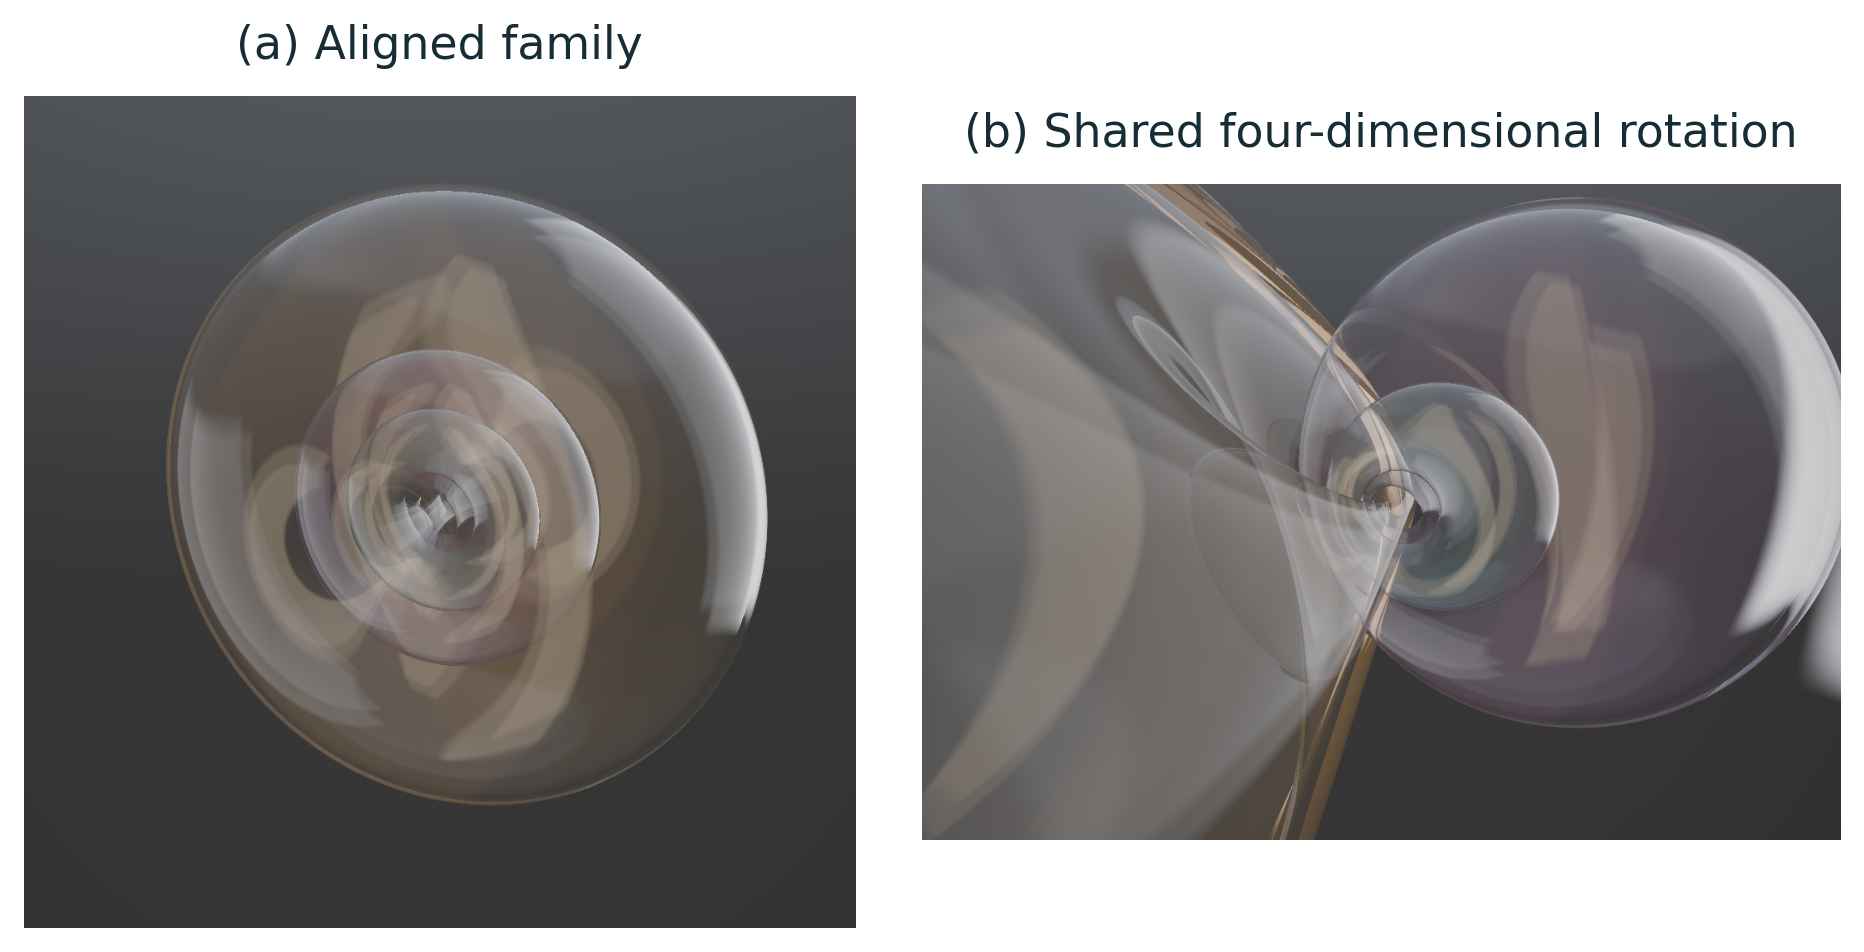
\includegraphics[width=1\linewidth,height=\textheight,keepaspectratio,alt={Three projected tori, with 0.5° angular shells, before and after a shared four-dimensional rotation. Both views are direct production-shader renders; camera, material and rotation settings are supplied with the software.}]{../technical-note/figures/three-tori.png}
\caption{Three projected tori, with 0.5° angular shells, before and
after a shared four-dimensional rotation. Both views are direct
production-shader renders; camera, material and rotation settings are
supplied with the software.}\label{fig:teaser}
}
\maketitle
\begin{abstract}
\small
We present a browser-based renderer for stereographic projections of
rotated Hopf tori, including solid regions and thin angular shells. A
rank-two projector supplies implicit quartic intersections and analytic
normals. The implementation study provides a homogeneous construction of
bounded ray charts for surfaces passing through infinity, a workflow
separating numerical failure stages, and comparisons of complete
refractive renderers. We evaluate the float32 implementation against an
independent exact-rational reference and an adapted Yuksel--Peters GPU
baseline. All three modern variants match the original 867-case corpus
at relative-distance tolerance \(10^{-4}\). A frozen, seeded 2,400-query
stress corpus exposes the same 109 grazing failures in each variant; all
1,800 other queries pass. Exact replay of captured GPU coefficients
reproduces those failures before root isolation. Independent checks of
selected optical paths retain thin-shell boundaries and Snell-law
refraction. Complete-render comparisons show close image agreement and
workload-dependent performance on Apple M3 Pro. Tangencies and
finite-precision polynomial construction remain explicit limitations.

\end{abstract}
\section{Motivation and scope}\label{motivation-and-scope}

A torus in the unit three-sphere can pass through the stereographic
projection pole while remaining a smooth compact surface in four
dimensions. Its three-dimensional image becomes unbounded and
subsequently appears to turn inside out. This geometry is established
\citep{banchoff1990, mccuan1998}. It provides a useful setting for
investigating how an interactive implicit renderer handles distant
intersections, changing material regions and closely spaced optical
boundaries.

This implementation study offers three reusable elements:

\begin{itemize}
\tightlist
\item
  \textbf{Bounded ray charts from a homogeneous implicit form.} Near and
  reciprocal coordinates cover the unbounded ray domain without a finite
  clipping sphere, with explicit handling of finite intersections and
  material boundaries through the projection pole (Sections 2 and 3).
\item
  \textbf{A workflow for separating numerical failures.} Independent
  references and intermediate captures distinguish input quantization,
  polynomial construction, root isolation and ray transport. This
  prevents an upstream construction error from being attributed to the
  root finder (Section 4).
\item
  \textbf{Comparisons of complete refractive renderers.} Shared scenes
  and transport settings connect intersection accuracy to boundary
  retention, image differences and rendering cost. The measured solver
  ranking changes with the optical workload (Section 4).
\end{itemize}

Hopf Observatory implements these elements in WebGL 2, with six-plane
\(SO(4)\) rotations, up to three torus regions, angular shells down to
\(0.01^\circ\), and projected Euclidean reflection/refraction. Figure~\ref{fig:teaser}
shows the family under a shared rotation. A fullscreen triangle
dispatches per-pixel ray calculations without tessellating the surface.

Ray tracing algebraic surfaces \citep{hanrahan1983}, GPU Bernstein
methods \citep{seland2007}, derivative-partitioned root finding
\citep{yuksel2022, peters2023}, and refinement against the original
implicit field \citep{szente2026} all predate this work. The
contribution is the concrete construction and evaluation workflow
supplied with this implementation. We claim neither a new general
root-finding algorithm nor superior root completeness over the modern
baseline. Reusing the approach for other implicit surfaces requires
evaluating their numerical thresholds and rendering workloads.

\section{Geometry and the projection
pole}\label{geometry-and-the-projection-pole}

The family in \(S^3\subset\mathbb R^4\) is \[
q(t,a,b)=(\cos t\cos a,\cos t\sin a,\sin t\cos b,\sin t\sin b)^T,
\quad 0<t<\pi/2.
\] For \(R\in SO(4)\), set \(P=R\,\mathrm{diag}(1,1,0,0)R^T\) and
\(c=\cos^2t\). A rotated torus satisfies \(q^TPq=c\). The six rotation
controls are redundant: \(SO(2)\times SO(2)\) stabilizes the original
projector, leaving four continuous rotational degrees of freedom at
fixed \(t\).

For \(p=(x,y,z)\), inverse stereographic projection is
\(Q(p)=V/(1+|p|^2)\), where \(V=(2p,|p|^2-1)^T\). Clearing the positive
denominator gives \[
f_c(p)=V^T(P-cI)V=0.
\] The exact gradient is \[
\nabla f_c=4\left[(PV)_{1:3}+p\big((PV)_4-c(1+|p|^2)\big)\right].
\] Its normalized direction supplies smooth surface normals.
Substituting \(p=o+sd\) gives a polynomial of degree at most four. Its
leading coefficient is \((P_{44}-c)|d|^4\). Thus the pole condition
\(P_{44}=c\) removes the quartic term; it does not justify discarding
all remaining finite intersections. A three-dimensional line lifts to a
circle through the projection pole in \(S^3\). The supplementary
technical note gives this construction and the full coefficient
derivation.

Figure~\ref{fig:pole} shows the projected surface on both sides of the pole
condition.

\begin{figure}[htbp]
\centering
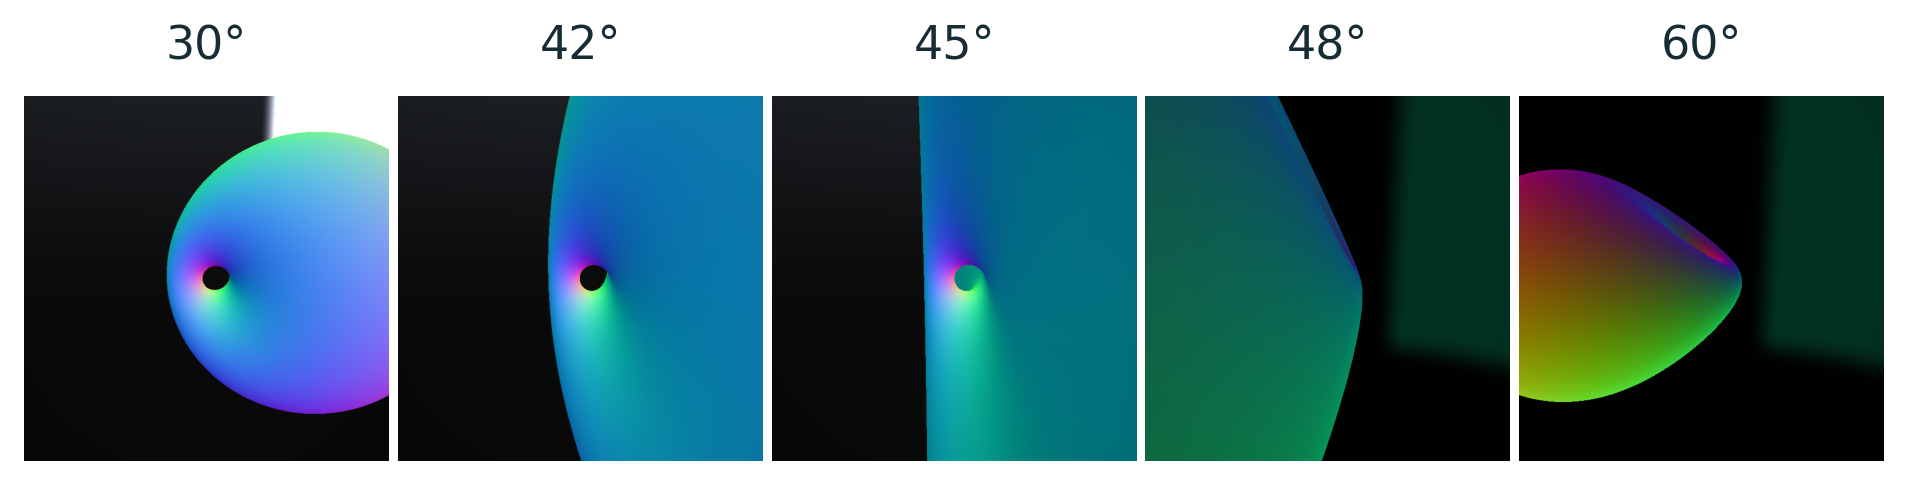
\includegraphics[width=1\linewidth,height=\textheight,keepaspectratio,alt={Passage through the projection pole for the 45° torus under XW rotations of 30°, 42°, 45°, 48° and 60°. Color encodes the production shader's analytic normal. The middle surface is unbounded; the views show a finite camera window, not a clipped geometric model.}]{../technical-note/figures/pole-sequence.png}
\caption{Passage through the projection pole for the 45° torus under XW
rotations of 30°, 42°, 45°, 48° and 60°. Color encodes the production
shader's analytic normal. The middle surface is unbounded; the views
show a finite camera window, not a clipped geometric
model.}\label{fig:pole}
\end{figure}

\section{Intersection and optical
implementation}\label{intersection-and-optical-implementation}

\subsection{Bounded ray charts}\label{bounded-ray-charts}

For unit \(d\), write \(k=o\cdot d\), \(C=o-kd\), \(\lambda=s+k\) and
\(L=\max(1,|C|)\). Each signed half-line uses a near coordinate
\(x=|\lambda|/L\in[0,1]\) and a reciprocal coordinate
\(x=L/|\lambda|\in(0,1]\). Let \(e=\sigma d\), with
\(\sigma\in\{-1,1\}\), and define \[
\begin{aligned}
a&=(2C/L^2,(|C|^2-1)/L^2)^T,\\
b&=(2e/L,2C\cdot e/L)^T,\qquad h=(0,0,0,e\cdot e)^T.
\end{aligned}
\] The near numerator is \(W(x)=a+bx+hx^2=V(C+Lxe)/L^2\). In the
reciprocal chart, multiplication by \(x^2\) reverses the coefficients:
\(W(x)=h+bx+ax^2=x^2V(C+Le/x)/L^2\). Both yield bounded polynomial
domains for \(g=W^T(P-cI)W\). The reciprocal endpoint \(x=0\) represents
infinity and is excluded from finite hits. Although \(C\cdot e=0\) and
\(e\cdot e=1\) in exact arithmetic, the shader retains their computed
values.

\Needspace{9\baselineskip}
For either chart, write \(W=u+vx+wx^2\), set \(w_0=u\), \(w_1=u+v/2\),
\(w_2=u+v+w\), and define \(B(a,b)=a^T(P-cI)b\). The quartic Bernstein
coefficients are constructed directly: \[
\begin{aligned}
b_0&=B(w_0,w_0), & b_1&=B(w_0,w_1),\\
b_2&=\bigl(B(w_0,w_2)+2B(w_1,w_1)\bigr)/3,\\
b_3&=B(w_1,w_2), & b_4&=B(w_2,w_2).
\end{aligned}
\] The scale \(L^{-2}\) limits coefficient growth before forming the
quadratic products. There is no division by a small leading monomial
coefficient at degree loss. In the reciprocal chart, relative
perturbations of \(x\) and \(|\lambda|=L/x\) have approximately equal
magnitude. This supplies a useful coordinate representation for distant
hits, without certifying that they can be resolved in float32.

\subsection{Isolation, refinement and
acceptance}\label{isolation-refinement-and-acceptance}

Derivative roots partition the quartic into monotone intervals. The
shader solves the derivative hierarchy from linear through quartic using
Bernstein coefficient differences and de Casteljau evaluation. A
strictly one-signed coefficient hull rejects a chart before isolation.
Sign-changing intervals receive at most 25 bisection steps followed by
interpolation within the final bracket. Exact endpoint zeros are
retained. Near-zero stationary values supply contact candidates only
when neither adjacent interval already contains a sign change.

After normalizing each polynomial by its maximum absolute coefficient,
the stationary-value threshold is
\(2.5\times10^{-7}E(x)+2\times10^{-9}\), where \(E\) evaluates the
polynomial with absolute Bernstein coefficients. This is the heuristic
called \passthrough{\lstinline!errorBound!} in the shader, not an
interval-arithmetic bound. The Bernstein solver consolidates successive
chart candidates within \(3\times10^{-7}\max(|x_i|,|x_j|)\). The
all-roots collector removes only identical float hit distances; it adds
no distance tolerance to the solver's internal candidate handling.
Distinct reference roots remain separately accountable.

Up to four Newton proposals evaluate the homogeneous form, with
\(g'=2(v+2xw)^T(P-cI)W\). A proposal must remain in \([0,1]\), move by
at most \(0.05\max(x,10^{-6})\), and strictly reduce the computed
\(|g|\). A rejected proposal retains the preceding candidate. This guard
does not certify distance accuracy or preserve the final isolation
bracket. With \(M=|W|^T|P-cI||W|\), using componentwise absolute values,
the final acceptance test is \[
\rho=\frac{|g|}{M+|g'|\,\eta}<2\times10^{-6},\qquad
\eta=\begin{cases}1&\text{near chart},\\x&\text{reciprocal chart}.\end{cases}
\] The code assigns zero residual when the denominator vanishes. A
finite converted distance beyond the self-intersection cutoff is also
required. The factor \(x\) in the reciprocal derivative term prevents a
fixed absolute tolerance from admitting increasingly inaccurate distant
roots.

Listing~\ref{lst:intersection} summarizes the nearest-boundary query. Each chart returns its
smallest accepted original-ray distance, regardless of the ordering of
its chart roots. A chart junction belongs to both charts; an identically
zero polynomial has no isolated crossing. The complete helpers are
\passthrough{\lstinline!chartVectors!},
\passthrough{\lstinline!chartPoly!},
\passthrough{\lstinline!quarticRoots!},
\passthrough{\lstinline!refineChart!} and
\passthrough{\lstinline!chartIntersection!} in
\passthrough{\lstinline!web/shader.js!}.

\begin{lstlisting}[caption={Nearest finite intersection with one boundary (Section~\ref{isolation-refinement-and-acceptance}).}, label=lst:intersection]
nearestBoundary(o, d, level, minS):
    k = dot(o, d); C = o - k*d; L = max(1, length(C))
    charts = [(+1, near), (+1, reciprocal)]
    if k < 0:
        prepend [(-1, reciprocal), (-1, near)] to charts
    for (sign, kind) in charts:
        W = chartVectors(C, sign*d, L, kind)
        b = bernsteinCoefficients(W, level)
        if all b > 0 or all b < 0: continue
        best = infinity
        for x in isolate(b):
            x = refineHomogeneous(W, level, x)
            if kind == reciprocal and x <= 0: continue
            distance = L*x if kind == near else L/x
            s = sign*distance - k
            if finite(s) and s > minS
               and residual(W, level, x, kind) < 2e-6:
                best = min(best, s)
        if best < infinity: return best
    return none
\end{lstlisting}

\subsection{Materials and finite-precision
transport}\label{materials-and-finite-precision-transport}

A solid fills \(Q^TPQ>c\). A shell is a band between distinct parameter
levels: \[
\cos^2(t+\Delta t/2)<Q^TPQ<\cos^2(t-\Delta t/2).
\] Its two boundaries are solved independently; their outward normals
have opposite signs. Angular width is measured in \(S^3\), not as
constant Euclidean thickness. Up to three regions share \(P\). Distinct
level surfaces do not intersect geometrically; their material bands may
overlap. The narrowest active level interval has priority, with a fixed
slot order breaking ties.

Each tracing step chooses the nearest enabled boundary, identifies the
incident and transmitted media, and applies Euclidean Snell refraction.
With incident unit direction \(d\) and opposing normal \(n\), let
\(\eta=n_1/n_2\), \(c_i=-d\cdot n\), and \(K=1-\eta^2(1-c_i^2)\). If
\(K\ge0\), the transmitted direction is \[
d_t=\eta d+(\eta c_i-\sqrt K)n;
\] otherwise the ray reflects internally. Interfaces hidden inside the
same effective medium do not refract.

Let \(\gamma\) be the smallest distinct angular boundary separation
among enabled regions, in radians. The bias scale is
\(\beta=\operatorname{clamp}(0.05\gamma,10^{-6},4\times10^{-4})\); a
lone solid uses the upper limit. The positive-distance cutoff is
\(\beta\max(1,|o|)/2\) and the post-hit offset is \(\beta\max(1,|p|)\).
This couples the offset to the boundary spacing and helps retain the
tested \(0.01^\circ\) walls, but cannot resolve arbitrarily thin
projected features. The main path allows at most 24 boundary iterations,
including skipped boundaries; the first reflected branch has a smaller
budget. Energy cutoffs, approximate environment reflections and
absorption in unbounded regions limit physical fidelity. There are no
caustics or full global illumination.

\section{Independent numerical
evaluation}\label{independent-numerical-evaluation}

All hardware measurements use Apple M3 Pro. Native tests execute the
production GLSL bodies through OpenGL 4.1 Metal, changing the version
directive from GLSL ES 3.00 to 4.10. Recorded browser validation uses
WebGL 2/ANGLE Metal on the same device; CI integration checks use
software WebGL. A second GPU is not part of this study.

The reference expands the original ray polynomial in exact rational
arithmetic and isolates its positive roots using SymPy's
continued-fraction method \citep{meurer2017}, with brackets no wider
than \(10^{-30}\). It imports no production intersection routines. One
reference uses the exact binary values of uploaded float32 inputs;
another uses the intended geometry serialized at 80 decimal digits, or
exact rationals for tangent constructions. These distinguish geometry
quantization from computation on the represented geometry.

We compare production Bernstein with an adaptation of Peters's CC0 GLSL
implementation \citep{peters2023} of Yuksel's method \citep{yuksel2022}.
The latter is evaluated in centered affine coordinates with a
coefficient-derived Cauchy bound, and in the same near/reciprocal
charts. Exact degree reduction, endpoint handling, iteration limits and
homogeneous refinement are shared between the two Yuksel variants. This
is an adapted GLSL baseline, not the author's complete optimized C++
library. Source provenance and modifications are recorded in the
supplement.

Each method enumerates all distinct positive roots of the unchanged
original ray, without origin advance, rendering bias or finite far
clipping. Maximum-cardinality one-to-one matching uses
\(|s_{\mathrm{GPU}}-s_{\mathrm{ref}}|/\max(1,|s_{\mathrm{ref}}|)\le\tau\).
A query fails if any root or output is unmatched. The collector
consolidates only identical float hit distances; the matching does not
merge nearby reference roots. Internal solver tolerances still apply,
and missing roots are reported alongside retained-root errors. Raw and
commonly refined outputs are retained.

\subsection{Fixed and seeded corpora}\label{fixed-and-seeded-corpora}

On the original 867 hand-designed cases, all three variants match all
1,470 reference roots at \(\tau=10^{-4}\), before and after refinement.
A conventional float32 Ferrari port fails on 378 cases after refinement;
this comparison is not evidence against every analytic solver.

The final stress corpus was constructed before its GPU evaluation, with
seed 20261121 and a frozen production revision. Its 2,400 boundary
queries include general random rays, targeted pole cases, rational exact
tangencies and small normal offsets, and 100 three-shell groups with six
boundary queries each. Rotation sampling uses six independent angle
draws, not Haar-uniform sampling on \(SO(4)\). The 600 grazing cases
comprise 200 exact intended double contacts and 400 nearby rays. All
shells have width \(0.01^\circ\); groups include separated and
overlapping bands and pole-crossing walls.

{
\Needspace{10\baselineskip}\begin{longtable}[]{@{}
  >{\raggedright\arraybackslash}p{(\linewidth - 8\tabcolsep) * \real{0.1579}}
  >{\raggedleft\arraybackslash}p{(\linewidth - 8\tabcolsep) * \real{0.2105}}
  >{\raggedleft\arraybackslash}p{(\linewidth - 8\tabcolsep) * \real{0.2105}}
  >{\raggedleft\arraybackslash}p{(\linewidth - 8\tabcolsep) * \real{0.2105}}
  >{\raggedleft\arraybackslash}p{(\linewidth - 8\tabcolsep) * \real{0.2105}}@{}}
\toprule\noalign{}
\begin{minipage}[b]{\linewidth}\raggedright
Family
\end{minipage} & \begin{minipage}[b]{\linewidth}\raggedleft
Queries
\end{minipage} & \begin{minipage}[b]{\linewidth}\raggedleft
Represented roots
\end{minipage} & \begin{minipage}[b]{\linewidth}\raggedleft
Input changes
\end{minipage} & \begin{minipage}[b]{\linewidth}\raggedleft
Failed queries
\end{minipage} \\
\midrule\noalign{}
\endhead
\bottomrule\noalign{}
\endlastfoot
Random & 600 & 861 & 0 & 0 \\
Pole & 600 & 501 & 253 & 0 \\
Grazing & 600 & 584 & 304 & 109 \\
Shell & 600 & 1,368 & 13 & 0 \\
\end{longtable}
}

Input changes count intended/represented root-set mismatches at
\(10^{-4}\). Failed-query counts apply to each refined modern variant,
on the same query IDs. These columns describe different comparisons and
must not be added.

All 1,800 non-grazing queries pass. Every solver retains boundary
ordering in all 100 shell groups. Bernstein matches 3,166 of the full
corpus's 3,314 represented roots, with 148 missing roots and 137
unmatched outputs; each Yuksel variant matches 3,165, with 149 missing
and 137 unmatched outputs. For each solver, the 109 failures comprise 40
output-count shortfalls, 34 excesses and 35 position failures despite
equal counts. An unmatched output may be an inaccurate root rather than
a wholly separate false intersection.

At \(\tau=10^{-5}\), refined failed-query counts are 197, 195 and 195
for Bernstein, centered Yuksel and chart Yuksel, respectively; at
\(10^{-6}\) they are 294, 292 and 292. Figure~\ref{fig:stress} shows the error-source
distinction and tolerance dependence. These aggregate counts alone do
not identify a causal stage; Section~\ref{post-hoc-diagnosis-of-grazing-failures} examines the construction and
solution stages separately.

\begin{figure}[htbp]
\centering
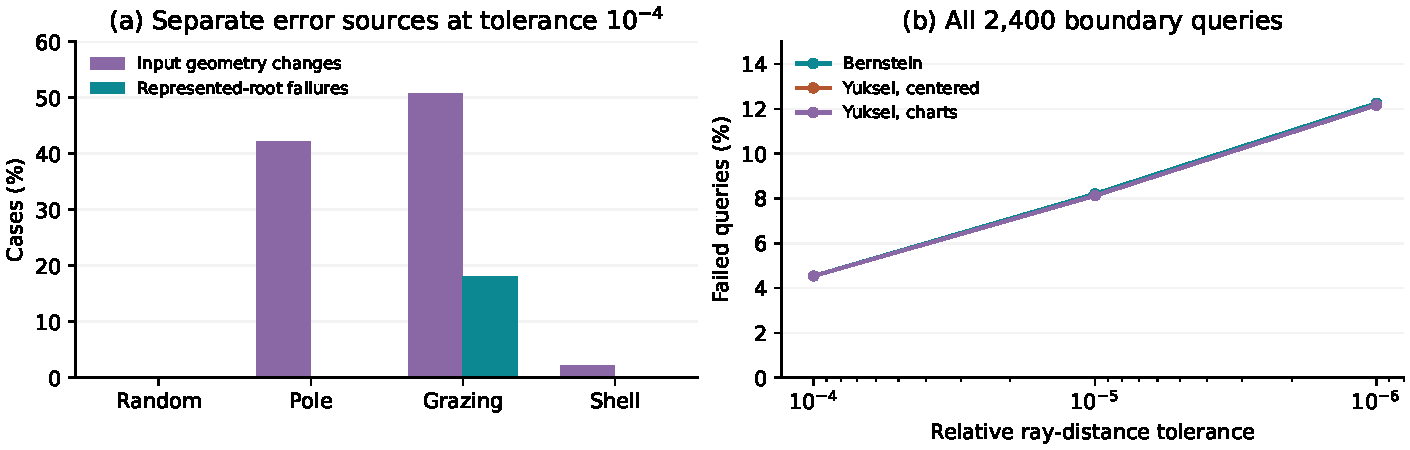
\includegraphics[width=1\linewidth,height=\textheight,keepaspectratio,alt={Stress validation. Left: input-geometry changes and represented-root failures at 10\^{}\{-4\}; the latter count is identical for all three methods. Right: failed queries as the tolerance tightens. Methods overlap substantially. All results use distinct-root matching without proximity consolidation.}]{../research/figures/stress-validation.pdf}
\caption{Stress validation. Left: input-geometry changes and
represented-root failures at \(10^{-4}\); the latter count is identical
for all three methods. Right: failed queries as the tolerance tightens.
Methods overlap substantially. All results use distinct-root matching
without proximity consolidation.}\label{fig:stress}
\end{figure}

For Bernstein, the largest nearest-returned-root ray-distance error is
\(7.98\times10^{-4}\), from grazing cases; missing roots have no finite
returned-root error. In the pole family the largest absolute position
difference is about 31.5 scene units at a hit roughly \(3.55\times10^8\)
units away. Both absolute and position-normalized errors are retained to
make that scale explicit. Float32 input rounding alone changes 570 query
root sets beyond the principal tolerance. A solver cannot recover an
intended distant root absent from the uploaded polynomial.

\subsection{Optical and image checks}\label{optical-and-image-checks}

Existing regressions pass 31 focused thin-shell cases and 36 transport
paths with 392 events. The \(0.01^\circ\) axis paths retain four entries
and four exits per single shell, and twelve of each across three shells.

Additionally, twelve predetermined paths from the seeded shell groups
are captured from each complete renderer. Exact-rational isolation
checks each captured incoming ray against all six represented
boundaries. Independent analytic normals, spatial medium probes and
scalar/vector Snell checks separate transport behavior from root
enumeration. Each variant passes 167 boundary events: 158 optical events
and nine hidden boundaries. One path reaches the 24-boundary cap and one
ends at the energy cutoff; these are recorded, not certified complete
paths. Other terminal misses are checked for remaining intersections.
Maximum hit-distance error is below \(3.97\times10^{-6}\) and maximum
Snell residual below \(9.30\times10^{-8}\) across these paths.

Five fixed scenes, in material, normal and depth modes at 480×270,
provide 30 paired image comparisons against Bernstein. Maximum
frame-mean absolute RGB8 error is \(2.82\times10^{-6}\) on a normalized
scale. One pixel in a centered-Yuksel solid render differs by more than
0.05, reaching 0.341; no other comparison exceeds 0.05 at any pixel.
These are close rendered outputs, not exact equivalence or independent
image ground truth.

\subsection{Rendering cost}\label{rendering-cost}

Full optical-renderer timings use three blocks of five warmup and ten
measured frames per variant/configuration, rotating variant order.
Native draw-plus-\passthrough{\lstinline!glFinish!} wall time excludes
compilation, readback, UI and vsync. Pooled medians at 1280×720 and a
24-boundary cap are:

{
\Needspace{10\baselineskip}\begin{longtable}[]{@{}lrrr@{}}
\toprule\noalign{}
Scene & Bernstein & Yuksel centered & Yuksel charts \\
\midrule\noalign{}
\endhead
\bottomrule\noalign{}
\endlastfoot
One solid & 3.13 ms & 2.86 ms & 2.88 ms \\
One 0.01° shell & 5.63 ms & 6.38 ms & 5.55 ms \\
Three 0.01° shells & 19.78 ms & 33.02 ms & 22.27 ms \\
Three shells, XW = 45° & 38.45 ms & 67.69 ms & 45.74 ms \\
\end{longtable}
}

The workload-dependent result supports retaining Bernstein for this
application's three-shell scenes. It establishes neither general solver
superiority nor a browser-speed or cross-vendor claim. Raw samples,
block medians and interquartile ranges remain available; small timing
differences should not be overinterpreted.

\subsection{Post-hoc diagnosis of grazing
failures}\label{post-hoc-diagnosis-of-grazing-failures}

We preserve the original experiment and diagnose all 600 grazing
queries, including its 491 passing controls. Separate GPU probes capture
the centered ray, homogeneous vectors, matrix subtraction, polynomial
coefficients, and candidates before and after refinement and filtering.
Exact-rational isolation then solves the captured intermediate
polynomials, with coordinate brackets no wider than \(10^{-40}\). Every
stage is compared with the original exact reference for the uploaded
float32 inputs at \(\tau=10^{-4}\). Thus this measures construction
error after upload, separately from intended-to-represented geometry
changes.

The first substitution solves the exact ray \(C+(s+k)d\) using captured
\(C\) and \(k\). The next two use captured \(W\) with, respectively,
exact and float32 subtraction in \(A=P-cI\). Finally we solve the
captured Bernstein or power coefficients exactly. All three methods give
the following query counts and failed-ID sets:

{
\Needspace{10\baselineskip}\begin{longtable}[]{@{}lrr@{}}
\toprule\noalign{}
Stage solved or observed & Failed / 600 & Of final 109 \\
\midrule\noalign{}
\endhead
\bottomrule\noalign{}
\endlastfoot
Exact reconstructed centered ray & 39 & 34 \\
Captured \(W\), exact \(A\) & 103 & 88 \\
Captured \(W\), rounded \(A\) & 106 & 90 \\
Exact roots of captured coefficients & 109 & 109 \\
GPU isolated candidates & 109 & 109 \\
Refined candidates, before filtering & 109 & 109 \\
Final accepted GPU roots & 109 & 109 \\
\end{longtable}
}

The last column counts the final failed queries already discrepant at
that stage. Intermediate sets are not nested, so differences between
rows are not additive error budgets. Nevertheless, exact solving of the
captured coefficients reproduces the entire final failure set and its 40
shortfalls, 34 excesses and 35 position failures. Improved isolation of
those polynomials alone cannot recover the original represented ray's
root set at this tolerance. Figure~\ref{fig:grazing} traces the original report's first
representative in each failure category.

\begin{figure}[htbp]
\centering
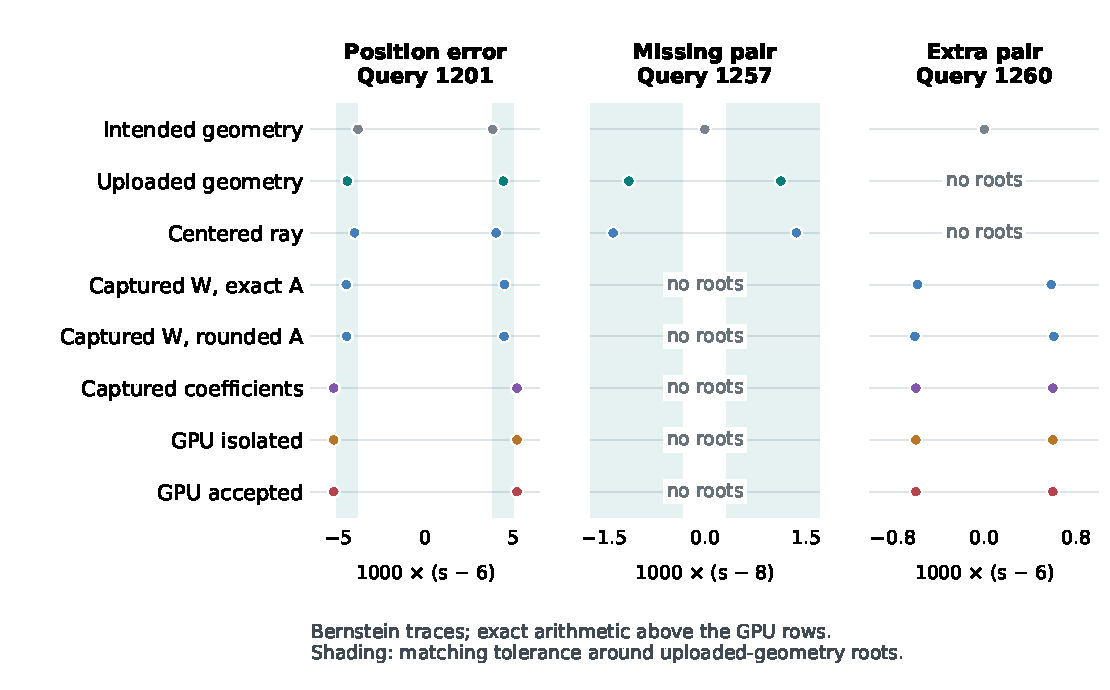
\includegraphics[width=1\linewidth,height=\textheight,keepaspectratio,alt={Grazing diagnostics for the three predetermined Bernstein representatives: position error, missing pair and extra pair. Rows above GPU isolation use exact arithmetic on the indicated representation. Shading marks the matching tolerance around uploaded-geometry roots. A pair can disappear or appear during chart construction, or shift beyond tolerance during coefficient construction. Other methods' traces are retained in the supplement.}]{../research/diagnostics/grazing/results/grazing-diagnostic.pdf}
\caption{Grazing diagnostics for the three predetermined Bernstein
representatives: position error, missing pair and extra pair. Rows above
GPU isolation use exact arithmetic on the indicated representation.
Shading marks the matching tolerance around uploaded-geometry roots. A
pair can disappear or appear during chart construction, or shift beyond
tolerance during coefficient construction. Other methods' traces are
retained in the supplement.}\label{fig:grazing}
\end{figure}

Removing Bernstein's internal proximity consolidation changes no raw or
refined output on these 600 queries. The residual filter rejects no
forward finite candidate. Refinement changes some positions and
matched-root counts, but no failed-query classification. Against the
captured coefficient roots, both Yuksel variants pass every query.
Bernstein differs on query 1311: a near-zero stationary candidate at
\(s=4\) is returned even though the captured polynomial has no real
roots. It matches one of the original ray's two roots within tolerance,
explaining the one-root aggregate difference without a completeness
advantage.

All 3,600 unchanged raw/refined replay outputs reproduce the frozen
float hit sets, as does the instrumented collector. Separate chart
probes differ by one ULP in three comparisons on two queries, with no
classification change; these discrepancies are retained. The study is a
post-hoc stage analysis on the same GPU, not fresh independent
validation or an instruction-level error attribution. Its protocol,
hashes, exact brackets, per-case traces and diagnostic-only ablation are
supplied in \passthrough{\lstinline!research/diagnostics/grazing/!}.

\section{Numerical limitations and implementation
lessons}\label{numerical-limitations-and-implementation-lessons}

The stress results distinguish three practical limits. First, the
intended surface may differ from the float32 surface supplied to the
GPU. Second, roots of the represented polynomial may be missed, merged
or positioned inaccurately. Third, a renderer may find individual
boundaries correctly but skip them after a finite origin offset or stop
before completing a path. Separate references and transport captures are
needed to distinguish these effects.

Near a tangent, a small perturbation can split a double root into two
crossings or remove the contact. A small residual then need not imply an
accurate distance, and a tolerance for accepting stationary values can
trade missing contacts against extra candidates. The diagnostic locates
all 109 principal-tolerance failures in the constructed coefficients
before isolation, while showing that earlier rounding errors can cancel
downstream. It motivates testing higher-precision construction or
refinement evaluated from the original ray inputs; neither remedy is
validated here. The deliberately grazing distribution is not an estimate
of failure frequency in ordinary viewing.

Refinement likewise requires measurement against geometric error. On the
original corpus's six-plane rotation subset, the largest Bernstein
relative-distance error is \(8.69\times10^{-7}\) without Newton
correction, \(1.23\times10^{-5}\) with unguarded step-limited
correction, and \(5.84\times10^{-6}\) with the production
residual-decrease guard. A conservative noise-aware guard leaves every
root unchanged on that corpus and forgoes improvements elsewhere. All
four policies still match the original corpus at \(10^{-4}\). These
results justify a limited safeguard, not a guarantee that polishing
improves accuracy.

For reuse, carry the original implicit form through coefficient
construction, candidate refinement and validation; retain raw candidates
as well as accepted hits. Test all roots of unchanged rays before
evaluating biased ray continuation. Report missing roots separately from
the errors of retained roots, and inspect both absolute and normalized
position errors for remote hits. Finally, compare complete shaders with
identical transport settings: the single-solid and three-shell timings
reverse the ranking of the centered baseline and Bernstein on this
device.

An unbounded chart domain does not provide unlimited numerical reach.
Float32 underflow, overflow, input quantization and finite offsets
remain relevant, and an identically zero polynomial represents a
contained line rather than an isolated crossing. The selected
\(0.01^\circ\) shell tests establish neither arbitrary path completeness
nor a minimum resolvable Euclidean thickness. More GPUs and independent
implementations would be needed to assess portability and generality.

\section{Conclusion and
reproducibility}\label{conclusion-and-reproducibility}

The implementation makes projected Hopf tori and thin-shell optics
interactively accessible, including passage through infinity.
Independent tests support the sampled non-grazing behavior and selected
optical paths. They also expose a substantial grazing failure rate:
109/600 deliberately difficult queries in every modern variant at
\(10^{-4}\). This replaces any broad robustness claim with a measured
domain of success and failure.

Exact replay of the captured grazing polynomials shows why solver
comparisons must include coefficient construction: all 109 failures
persist even with exact root isolation. These results support an
implementation study of this family, not a general root-completeness or
cross-device performance claim. The independent stress corpus and
selected transport captures delimit what has been checked.

The companion package's \passthrough{\lstinline!REVIEW.md!} is the entry
point. \passthrough{\lstinline!PAPER.md!} is this manuscript;
\passthrough{\lstinline!TECHNICAL\_NOTE.md!} contains the complete
derivation and implementation discussion;
\passthrough{\lstinline!research/STRESS.md!} and
\passthrough{\lstinline!research/README.md!} give seeds, provenance,
commands and limitations. Raw inputs, exact brackets, all outputs,
representative failures, rendered comparisons and a SHA-256 package
manifest are included. The buildless WebGL application runs with
\passthrough{\lstinline!npm start!}.

\section*{Assistance and
responsibility}\label{assistance-and-responsibility}
\addcontentsline{toc}{section}{Assistance and responsibility}

Tom Crosby supplied the geometric motivation, directed the project and
is responsible for the conclusions. OpenAI Codex assisted with
derivation, implementation, experiments, literature checking and
writing. The recorded independent references and tests verify results
within their stated scope. Codex is an AI tool, not a human author.
Figures are deterministic outputs of the supplied code.

\small
\bibliographystyle{jcgt}
\bibliography{references}
\section*{Index of supplemental
materials}\label{index-of-supplemental-materials}
\addcontentsline{toc}{section}{Index of supplemental materials}

\begin{itemize}
\tightlist
\item
  \passthrough{\lstinline!web/!}: WebGL 2 application, with
  intersections and optics in \passthrough{\lstinline!shader.js!}.
\item
  \passthrough{\lstinline!technical-note/technical-note.pdf!}: extended
  derivations and experiments.
\item
  \passthrough{\lstinline!research/README.md!}: protocols, dependencies,
  frozen results, exact references, transport captures, timings and
  generated figures.
\item
  \passthrough{\lstinline!research/diagnostics/grazing/!}: post-hoc
  captures, exact replays, ablation and frozen-evidence manifest.
\item
  \passthrough{\lstinline!REVIEW.md!},
  \passthrough{\lstinline!research/THIRD\_PARTY.md!} and
  \passthrough{\lstinline!LICENSE!}: review instructions and software
  provenance; the archive includes
  \passthrough{\lstinline!MANIFEST.json!}.
\end{itemize}

\section*{Author contact information}
Tom Crosby\\
\href{mailto:twcrosbynz@gmail.com}{twcrosbynz@gmail.com}
\end{document}
